\documentclass[svgnames,smaller,table]{beamer}
\usepackage{multirow}
\usepackage{tikz}
\usefonttheme[onlymath]{serif}

\usepackage{listings}
% Configura o listings
\lstset{
  %  basicstyle=\footnotesize,\small,...\tiny
  basicstyle=\ttfamily\scriptsize,
  commentstyle=\color{mygreen},
  numbers=left,
  stepnumber=1,
  showstringspaces=false,
  tabsize=2,
  breaklines=true,
  breakatwhitespace=false
 columns=fixed,
 fontadjust=true,
 basewidth=0.5em
}


\usetheme{lthn}
\setbeamercolor*{normal text}{fg=black}
% -----------------------------------------------------------------------------------------------------------------

\title[Slide]{The Use of Serpent at the LTHN/CDTN}
\author{Vitor Vasconcelos A. Silva}
\date{\today}
\institute{%
  LTHN - Thermal-hydraulics and Neutronics Laboratory
  \par
  Reactors Technology Service - CDTN/CNEN}

\begin{document}

%-------------------------------------------------
\begin{frame}
\titlepage
\end{frame}

%-------------------------------------------------
\begin{frame}
  \frametitle{Summary}
  \tableofcontents%[pausesections]
\end{frame}


\section{CDTN}
%-------------------------------------------------
\begin{frame}
  \frametitle{CDTN}
  \framesubtitle{Nuclear Technology Development Center}
  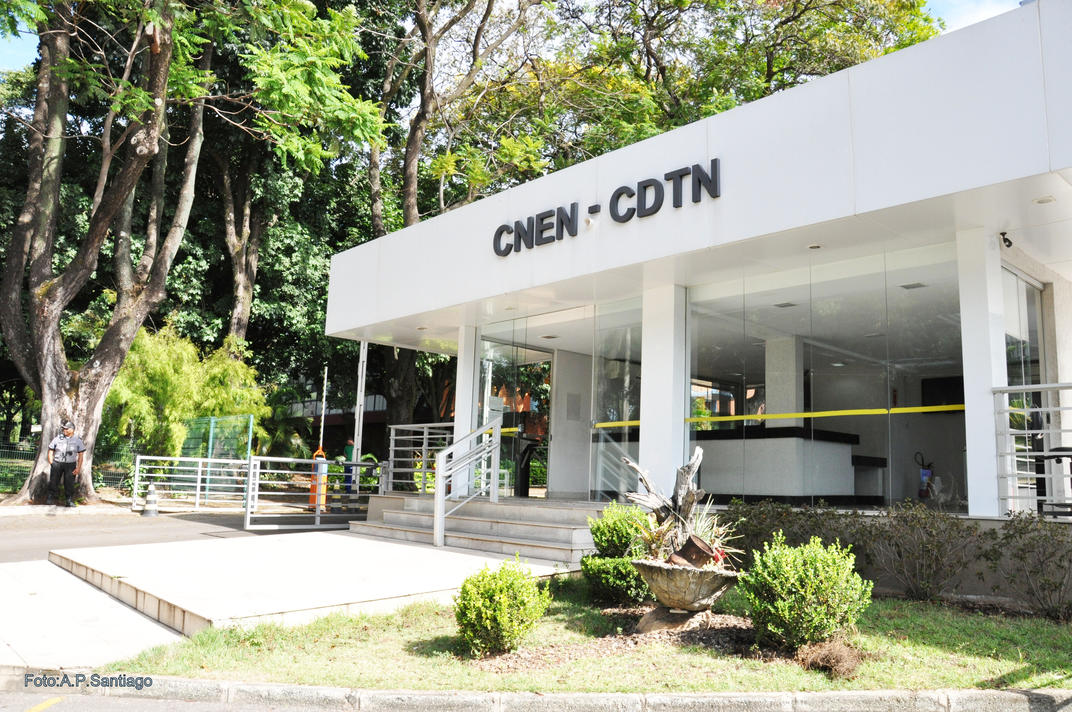
\includegraphics[scale=0.07]{figuras/portaria1_CDTN.jpg}
\end{frame}

%-------------------------------------------------
\begin{frame}
  \frametitle{CDTN}
  \framesubtitle{Nuclear Technology Development Center}
  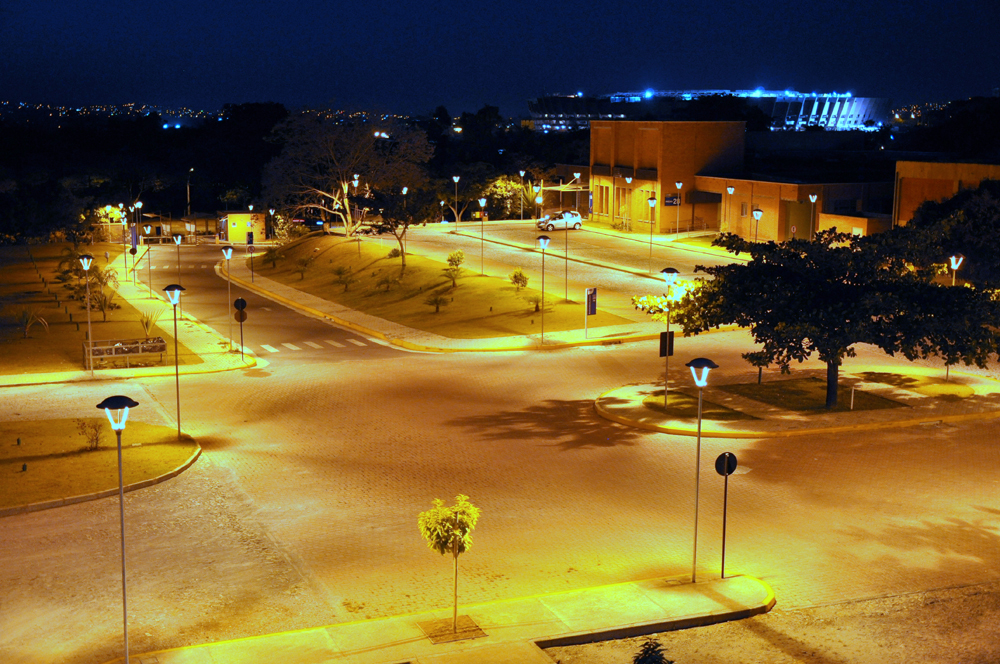
\includegraphics[scale=1.3]{figuras/predio_28_noite.jpg}
\end{frame}

%-------------------------------------------------
\begin{frame}
  \frametitle{CDTN}
  \framesubtitle{Nuclear Technology Development Center}
  \begin{itemize}
  \item Founded in 1952 as IPR (Radioactive Research Institute), part of
    Minas Gerais Federal University.
  \item In 1960, TRIGA Mark 1 reactor inaugurated - first criticality.
  \item Many areas...
    \item Neutronics + thermal....
      \end{itemize}
  \textbf{What do we have today?}
  \begin{itemize}
  \item New Strategic Plan (2019-2022) wants to promote reactor's modernization and \textit{use}
    \pause
    \item $\rightarrow$ ``new'' applications like \textbf{neutron imaging}. 
  \end{itemize}
\end{frame}


\section{LTHN}
%-------------------------------------------------
\begin{frame}
  \frametitle{TRIGA IPR-R1 Reactor}
  \framesubtitle{Characteristics}
  \begin{center}
    \begin{itemize}
    \item General Atomics Research Reactor, pool type.
    \item Licensed to operate at 100 kW\footnote{Operated at 250 kW under temporary authorization.}.
    \item LEU fuel, 59 aluminum and 4 stainless steel fuel elements.
    \end{itemize}
  \end{center}
\end{frame}

%-------------------------------------------------
\begin{frame}
  \frametitle{TRIGA IPR-R1 Reactor}
  \framesubtitle{Reactor pool, core and neutron extractor}
  \begin{center}
%    \includegraphics[scale=0.2]{figuras/extrator-poco.jpg}
    Figura?
  \end{center}
\end{frame}

\subsection{Neutrongraphy on TRIGA IPR-R1}
%-------------------------------------------------
\begin{frame}
  \frametitle{Neutrongraphy on TRIGA IPR-R1}
  \framesubtitle{The pioneers}
  \textbf{Brief historical background}
    \begin{itemize}
    \item 1970's, first ideas on the possible construction of a neutron extractor.
    \item 1987, the neutron extractor is installed into the reactor's pool.
    \item 2003, last use for neutrongraphy.
    \end{itemize}
    \vspace{10px}
  \textbf{Fabrication characteristics}
    \begin{itemize}
    \item 525 cm long aluminum tube.
    \item Made of 10 and 15 cm diameters tubes.
    \item A shield made of borated paraffin, lead, cadmium and steel was constructed to be connected to the top of the extractor.
    \end{itemize}
\end{frame}

\section{Neutron Extractor}
%-------------------------------------------------
\begin{frame}
  \frametitle{Neutron Extractor}
  \framesubtitle{Schematic}
  \begin{center}
%    \includegraphics[scale=0.2]{figuras/esquema.png}
    Outra figura?
  \end{center}
\end{frame}

%-------------------------------------------------
\begin{frame}
  \frametitle{Neutron Extractor}
  \framesubtitle{View}
  \begin{center}
%    \includegraphics[scale=0.2]{figuras/extrator1-original.jpg}
    Figura de novo.
  \end{center}
\end{frame}

%-------------------------------------------------
\begin{frame}
  \frametitle{Neutron Extractor}
  \framesubtitle{Closer view}
  \begin{center}
%    \includegraphics[scale=0.2]{figuras/extrator-zoom.jpg}
    Chega de figuras
  \end{center}
\end{frame}

%-------------------------------------------------
\begin{frame}
  \frametitle{Neutron Extractor}
  \framesubtitle{Technical aspects related to neutrongraphy}
    \begin{itemize}
    \item Collimation ratio: \scalebox{1}{$\left(\frac{L}{D}\right)=\frac{460cm}{10cm}=46$}
    \item Neutron to gamma ratio: \scalebox{1.5}{$\frac{n}{\gamma}$} $ = 153 \times 10^4 (mR)^{-1}.cm^{-2}$ \textsuperscript{[}\footnote{A. L. Costa, 2003}\textsuperscript{]} 
    \item Only one report on thermal/epithermal neutrons (Cd) ratio: at 3.6 meters over reactor's graphite reflector it is $27$. (Information only) 
    \end{itemize}
%    \vspace{10px}
\end{frame}

\section{Perspectives}
%-------------------------------------------------
\begin{frame}
  \frametitle{Perspectives}
  \framesubtitle{Explore (not so) new applications: neutron imaging}
  \textbf{More questions than answers}\\
  \vspace{10px}
  The state-of-the art: is TRIGA IPR-R1 capable of neutron imaging applications?\\
  \begin{itemize}
  \item Digital ``neutrongraphy''. (?)
  \item Neutron ``tomography''. (?)
  \item Historical art research. (?)
  \item Non-destructive tests. (?)
  \end{itemize}
\end{frame}

\section{Conclusions}
%-------------------------------------------------
\begin{frame}
  \frametitle{Conclusions}
  \framesubtitle{Resume neutron beam utilization}
  The first step on evaluating the capabilities of TRIGA IPR-R1 for neutron imaging applications, is to \textit{know} what are the current state-of-the-art applications and its technical aspects.\\
  \vspace{10px}
  ''\textit{Not-capable}'' is a perfect valid answer.\\
  \vspace{10px}
  \pause
  \textbf{But \textit{only} after the homework is done.}
\end{frame}



%-------------------------------------------------
% FIM
%-------------------------------------------------
\begin{frame}
 \vfill
  \begin{beamercolorbox}[center]{title}
     \Huge{Thank you!}
  \end{beamercolorbox}
  \vfill
\end{frame}


\end{document}

